% This is all the tagged PDF stuff:
%https://latex3.github.io/tagging-project/documentation/prototype-usage-instructions.html
% Uncomment if you can, but it will break: all verbatim environments (e.g. code), some templates (e.g. acm) etc.
%% \DocumentMetadata{
%%   lang        = en,
%%   pdfversion  = 2.0,
%%   pdfstandard = ua-2,
%%   pdfstandard = a-4f, %or a-4
%%   testphase   =
%%    {phase-III,
%%     title,
%%     table,
%%     math,
%%     firstaid}  
%% }

\documentclass[10pt, twocolumn]{IEEEtran}

\usepackage{lipsum}

\usepackage{mathptmx}
\usepackage{amsmath}
\usepackage{enumitem}
\usepackage{multirow}
\usepackage{subcaption}
\usepackage{url}

\usepackage{comment}
\usepackage{pifont}

\usepackage{color}
\usepackage{xspace}
\usepackage{booktabs,tabularx}
\usepackage[numbers,sort]{natbib}
\usepackage{ragged2e}
\usepackage{tikz}
\usepackage{dcolumn}
\usepackage{dsfont}
\usepackage{graphicx}
%\graphicspath{ {./images/} }

\usepackage{listings}
\usepackage{tcolorbox}
\usepackage{xcolor}
\usepackage{enumitem}
\usepackage{etoolbox}

\usepackage{hyperref}
\usepackage{flushend}
\usepackage{siunitx}

\usepackage[linesnumbered]{algorithm2e}
\SetAlCapFnt{\footnotesize}
\SetAlCapNameFnt{\footnotesize}
\SetAlCapSkip{4pt}

% Put all our special nonsense in here
\usepackage{localmacros}

\begin{document}

\title{Its a paper title}

% Trick for getting numbers into superscripts on names
\DeclareRobustCommand*{\IEEEauthorrefnum}[1]{\raisebox{0pt}[0pt][0pt]{\textsuperscript{\footnotesize\ensuremath{#1}}}}

% Note this author block has co-first authors, only relevant to some papers
\author{
\IEEEauthorblockN{
Co-Author 1\IEEEauthorrefnum{1}\IEEEauthorrefmark{1},
Co-Author 1\IEEEauthorrefnum{1}\IEEEauthorrefmark{2},
Author 2\IEEEauthorrefmark{1},
Author 3\IEEEauthorrefmark{2}\\
}
\IEEEauthorblockA{
\IEEEauthorrefmark{1}University of Washington,
\IEEEauthorrefmark{2}School 2\\
\{emails\}@cs.washington.edu,
\{emails\}@school2.edu
}
}
\clubpenalty=10000
\widowpenalty=10000

\maketitle
\footnotetext[1]{The two first authors contributed equally to the paper.}

\begin{abstract}
This is a paper abstract.
\end{abstract}

\section{Introduction}

Security is difficult to get right~\cite{kohlbrenner-shacham:fuzzyfox:usec16,kocher:timing-attacks:c96}.

\lipsum[2-10]

\section{Design}

\begin{figure}
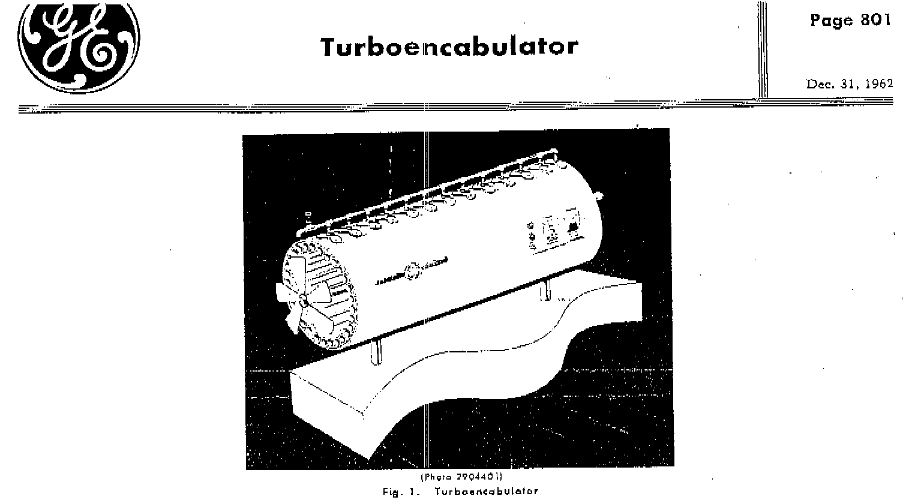
\includegraphics[width=\columnwidth,alt={The turboencabulator: a large cylindrical wonder-machine.}]{figures/design_diagram.png}
\caption{The caption.}
\label{fig:design_diagram}
\end{figure}
We have a very good design, as shown in Figure~\ref{fig:design_diagram}.

\input{text/acks}

\bibliographystyle{IEEEtran}
\bibliography{bibs/dkohlbre}

\end{document}
